\scanpage{32}\mspage{31}
% @ top, continuation lines 1–3
Si $A\in \unsure{F|\mathcal F}\setminus G$, $A\cap B$ est réunion de strates de $F$. \deleted{Reste} reste à voir que une strate \inserted{\unsure{$G$|$\in$}} de $F$ est réunion de strates de $F'$. Soit $A$ cette strate de $F$. \deleted{\unsure{On}}
% @ top, cancelled union
\[
 \deleted{A=\bigcup_{\substack{B\in F\\B\leq F}}B^\circ}
\]
% @ upper part, two cases; both high primes in the first case are visible
Si $A\notin G'$, alors $A\in F\setminus G'\subset F'$, et on gagne. Si $A\in G$, alors (comme $G'\preceq G$) $A$ est réunion de strates de $G'$, qui sont des strates de $F'$, et on gagne encore.

% @ left beside corollary
% slanted
\margin{Ultra faux}
% @ upper middle, corollary heading
\uline{Corollaire} Le \deleted{raffinement}\inserted{subdivision} précédente $F'$ de $F$ est caractérisée par \inserted{chacune} des propriétés équivalentes suivantes~:

% @ centre, condition a crossed by a large X
\deleted{a) Pour toute subdivision $F''$ de $F$ qui induit $G'$ sur $G$, on a $F''\preceq F'$ -- i.e. $F'$ est \deleted{\uline{maximal}}\inserted{un plus grand \unsure{élémt|élément|élt}} pour $\preceq^{*}$, dans l'ens des subdivisions de $F$ qui induisent $G'$ sur $G$.}
% @ small isolated angular mark directly below qui in the last long line of a
% The mark is reproduced graphically; its lexical role (E/in-like) is uncertain.
\figure{
\begin{tikzpicture}[x=1cm,y=1cm,line cap=round,line join=round]
\draw[line width=.7pt] (0,.43) -- (0,.03) .. controls (.04,-.01) and (.15,.01) .. (.33,.02);
\draw[line width=.6pt] (.10,.15) .. controls (.19,.19) and (.26,.18) .. (.35,.18);
\draw[line width=.2pt] (.05,.40) .. controls (.17,.44) and (.24,.42) .. (.33,.39);
\end{tikzpicture}}
% @ left of a, starred gloss
% slanted
\margin{$*$ ou pour $\ll$, cela revient au $=$ parmi des subdivisions d'une $=$ $F$}
% @ centre left, long oblique note
% slanted
% A long curved stroke crosses successive words. Whole-note cancellation is uncertain.
\margin{\deleted{les conditions \deleted{\unsure{a)}} b) c) d) sont équivalentes, \unsure{et} \uline{impliquées} par a), \unsure{lesquelles|laquelle} \unsure{caractérisent|caractérise} la subdivision construite \unsure{précédemm\textsuperscript{t}|précédemment}. Mais ces trois \unsure{cond.} (b,c,d) sont \unsure{loin} d'impliquer a)}}
% @ lower middle, condition b
b) L'application can. associée à $F'\preceq F$
\[
 \varphi:F'\longrightarrow F
\]
induit une bijection
% @ lower middle, bijection
\[
 F'\setminus G'\xrightarrow{\sim}F\setminus G.
\]
% @ right, NB; a vertical bracket stands to its left
\margin{\figure{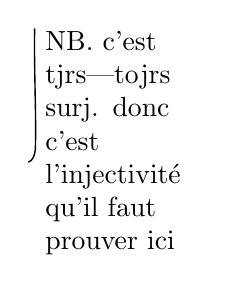
\begin{tikzpicture}[x=1cm,y=1cm]
\node[anchor=north west,inner sep=0pt,text width=2cm] at (0,0) {NB. c'est \unsure{tjrs|tojrs} surj. donc c'est l'\uline{injectivité} qu'il faut prouver ici};
\draw[line width=.5pt] (-.13,.03) .. controls (-.14,-.45) and (-.11,-1.05) .. (-.12,-1.46) .. controls (-.12,-1.57) and (-.15,-1.65) .. (-.21,-1.67);
\end{tikzpicture}}}
% @ lower part, condition c
c) \deleted{Les strates ouvertes de $F'$ qui ne sont} \inserted{$\forall A\in F\setminus G$, $A^\circ$ est une strate ouverte} de $F'$.

% @ lower part, condition d
d) $F'\supset F\setminus G$, i.e. $\forall A\in F\setminus G$, on a $A\in F'$.

% @ foot, proof heading; one live On, its opening stroke meets the heading underline
% Two tiny isolated pen marks between On and va have no recoverable lexical content.
\uline{Dém} On va prouver p. ex
% @ foot, cycle of implications
\[
 \text{d)}\Longrightarrow\text{b)}\Longrightarrow\text{c)}\Longrightarrow\text{a)}\Longrightarrow\text{d)}
\]
% @ bottom, first implication
\deleted{\uline{Dém}} $\text{d)}\Rightarrow\text{b)}$ Si $(F\setminus G)\subset F'$, alors $\varphi\mid F\setminus G$ est l'\deleted{\unsure{identité}}inclusion \deleted{(trivial)} \inserted{can. $F\setminus G\hookrightarrow F$}, \deleted{donc} donc il reste à prouver
% @ bottom edge, equality
\[
 F\setminus G=F'\setminus G'.
\]
